% Created 2024-01-30 Tue 15:43
% Intended LaTeX compiler: pdflatex
\documentclass[smaller]{beamer}\usepackage{listings}
\usepackage{color}
\usepackage{amsmath}
\usepackage{array}
\usepackage[T1]{fontenc}
\usepackage{natbib}
\lstset{
keywordstyle=\color{blue},
commentstyle=\color{red},stringstyle=\color[rgb]{0,.5,0},
literate={~}{$\sim$}{1},
basicstyle=\ttfamily\small,
columns=fullflexible,
breaklines=true,
breakatwhitespace=false,
numbers=left,
numberstyle=\ttfamily\tiny\color{gray},
stepnumber=1,
numbersep=10pt,
backgroundcolor=\color{white},
tabsize=4,
keepspaces=true,
showspaces=false,
showstringspaces=false,
xleftmargin=.23in,
frame=single,
basewidth={0.5em,0.4em},
}
\usepackage{natbib, dsfont, pgfpages, tikz,amssymb, amsmath,xcolor}
\bibliographystyle{abbrvnat}
% New operators and commands
\newcommand{\Z}{\mathbb{Z}}
\newcommand{\Q}{\mathbb{Q}}
\newcommand{\R}{\mathbb{R}}
\newcommand{\N}{\mathbb{N}}
\newcommand{\C}{\mathbb{C}}
\renewcommand{\S}{\mathbb{S}}
\newcommand{\blank}{\makebox[1ex]{\textbf{$\cdot$}}}
\newcommand\independent{\protect\mathpalette{\protect\independenT}{\perp}}
\def\independenT#1#2{\mathrel{\rlap{$#1#2$}\mkern2mu{#1#2}}}
\renewcommand{\phi}{\varphi}
\renewcommand{\epsilon}{\varepsilon}
\newcommand*\diff{\mathop{}\!\mathrm{d}}
\newcommand{\weakly}{\rightsquigarrow}
\newcommand\smallO{
  \mathchoice
    {{\scriptstyle\mathcal{O}}}% \displaystyle
    {{\scriptstyle\mathcal{O}}}% \textstyle
    {{\scriptscriptstyle\mathcal{O}}}% \scriptstyle
    {\scalebox{.6}{$\scriptscriptstyle\mathcal{O}$}}%\scriptscriptstyle
}
\newcommand{\midd}{\; \middle|\;}
\newcommand{\1}{\mathds{1}}
\usepackage{ifthen} %% Empirical process with default argument
% \newcommand{\G}[1][]{%
%    \ifthenelse{ \equal{#1}{} }
%       {\ensuremath{\mathbb{G}_n}}
%       {\ensuremath{\mathbb{G}_{#1}}}
% }
% New version:
\newcommand{\G}[2][n]{
{\ensuremath{\mathbb{G}_{#1}}{\left[#2\right]}}
}
\DeclareMathOperator*{\argmin}{\arg\!\min}

% New operators for consistent notation
\newcommand{\V}{\mathrm{Var}} % variance
\newcommand{\measure}[1]{\mathrm{{#1}}} % measure
% \newcommand{\measure}[1]{\textnormal{\textbf{{#1}}}} % measure
\newcommand{\m}[1]{\measure{#1}} % measure shortcut
\newcommand{\eqd}{\stackrel{d}{=}} % equality in distribution
\newcommand{\arrow}[1]{\xrightarrow{\; {#1} \;}}
\newcommand{\arrowP}{\xrightarrow{\; \m{P} \;}} % convergence in probability
\newcommand{\leb}{\lambda} % the Lebesgue measure
\newcommand{\T}{\top} % transpose
\newcommand{\KL}{\ensuremath{D_{\mathrm{KL}}}}

\usepackage{xargs}
% Make it easy to change counterfactual notation:
\newcommandx{\cf}[4][3={}, 4={}]{
  % \ifthenelse{ \equal{#4}{} }
  % {{#1^{#2}}(#3)}
  {\ifthenelse{ \equal{#3}{} }
    {{#1^{#2}}_{#4}}
    {{#1^{#2}}_{#4}(#3)}}
}

% Easily change notation:
\DeclareMathOperator{\TT}{\Psi} % target parameter
\newcommand{\lp}{\mathcal{L}_{\P}^2} % shortcut for lp2 space
\newcommand{\empmeas}{\hat{\mathbb{P}}_n} % empirical measure
\DeclareMathOperator{\E}{\mathbb{E}} % expectation
\renewcommand{\P}{\m{P}} % probability
\newcommand{\ic}{\mathrm{IF}} % influence curve
\definecolor{bblue}{rgb}{0.2,0.2,0.7}
\usepackage{prodint}
\setbeamertemplate{footline}[frame number]
\beamertemplatenavigationsymbolsempty
\usepackage{appendixnumberbeamer}
\setbeamercolor{gray}{bg=white!90!black}
\setbeamertemplate{itemize items}{$\circ$}
\lstset{basicstyle=\ttfamily\footnotesize}
\RequirePackage{fancyvrb}
\DefineVerbatimEnvironment{verbatim}{Verbatim}{fontsize=\footnotesize}
\makeatletter
\def\@fnsymbol#1{\ensuremath{\ifcase#1\or \dagger\or \ddagger\or
\mathsection\or \mathparagraph\or \|\or \dagger\dagger
\or \ddagger\ddagger \else\@ctrerr\fi}}
\makeatother
\renewcommand*{\thefootnote}{\fnsymbol{footnote}}
\AtBeginEnvironment{frame}{\setcounter{footnote}{0}}

\renewcommand*\familydefault{\sfdefault}
\itemsep2pt
\usepackage[utf8]{inputenc}
\usepackage[T1]{fontenc}
\usepackage{graphicx}
\usepackage{longtable}
\usepackage{wrapfig}
\usepackage{rotating}
\usepackage[normalem]{ulem}
\usepackage{amsmath}
\usepackage{amssymb}
\usepackage{capt-of}
\usepackage{hyperref}
\usetheme{default}
\author{Anders Munch \newline \small joint work with Thomas Gerds}
\date{January 30, 2024}
\title{The state learner \newline \normalsize a super learner for right-censored data}
\begin{document}

\maketitle
\section{Super learning with right-censored data}
\label{sec:orgdd3c161}
\begin{frame}[label={sec:org7c16a81}]{Setting and motivation}
Construct a targeted estimator of a low-dimensional target parameter such as the
average treatment effect.

\vfill

Available data are right-censored.

\vfill

Requires estimation of high-dimensional nuisance parameters such as the
conditional survival and censoring mechanism.

\vfill

Use super learning to alleviate the need to fully pre-specify estimators of the
nuisance parameters.

\vfill

\color{bblue}Challenge\color{black}: Existing super learners restrict which
learners can be included in the library or require pre-specification of an
estimator of the censoring mechanism.
\end{frame}

\begin{frame}[label={sec:org539d390},fragile]{Super learning\footnote{\cite{stone1974cross,geisser1975predictive,wolpert1992stacked,breiman1996stacked,van2007super}}}
 \small

Need to estimate the parameter
\begin{equation*}
  f = \argmin_{f \in \mathcal{F}} P{[L(f, \blank)]}, 
\end{equation*}
using the data set \( \mathcal{D}_n = \{O_1, \dots, O_n\} \).

\vfill

\begin{description}
\item[{Learner}] algorithm \(a\) that produces estimates, \(\mathcal{D}_n \mapsto
  a(\mathcal{D}_n) = \hat f_n\)
\item[{Library}] collection of learners, \(\mathcal{A} = \{a_1, a_2, \dots, a_M
  \}\)
\item[{Loss function}] \(L \colon \mathcal{F} \times \mathcal{O} \rightarrow \R\)
\end{description}

\vfill

Combine learners from the library into a new learner with performance almost as
good as the best of them.

\vfill

\color{bblue}Regression example\color{black}: \(L(f, O) =(f(X) -Y)^2\),
library consiting of the learners \texttt{lm}, \texttt{glm}, \texttt{glmnet}, \texttt{rfsrc}, \ldots{}
\end{frame}

\begin{frame}[label={sec:orga8ac7a8}]{Discrete super learner}
\small

\begin{description}
\item[{Learner}] algorithm \(a\) that produces estimates, \(\mathcal{D}_n \mapsto
  a(\mathcal{D}_n) = \hat f_n\)
\item[{Library}] collection of learners, \(\mathcal{A} = \{a_1, a_2, \dots, a_M \}\)
\item[{Loss function}] \(L \colon \mathcal{F} \times \mathcal{O} \rightarrow \R\)
\end{description}

\vfill

The discrete super learning is the data-adaptive learner
\begin{equation*}
  \hat{a}_n = \argmin_{a\in\mathcal A}\hat{R}_n(a; L),
\end{equation*}
where
\begin{equation*}
  \hat{R}_n(a; L) =
  \frac{1}{K}\sum_{k=1}^{K}
  \frac{1}{| \mathcal{D}_n^{k} |}\sum_{O_i \in \mathcal{D}_n^{k}}
  L
  {
    \left(
      a{ (\mathcal{D}_n^{-k})}
      , O_i
    \right)
  },
  \quad \text{with} \quad
  \mathcal{D}_n^{-k} = \mathcal{D}_n \setminus \mathcal{D}_n^{k}.
\end{equation*}
\end{frame}

\begin{frame}[label={sec:org5f30ed7}]{Right-censored data}
\small

\begin{block}{Notation}
\begin{description}
\item[{\color{black}\(X\)}] vector of baseline covariates
\item[{\(T\)}] time to event variable, \(T > 0\)
\item[{\(C\)}] censoring time, \(C > 0\)
\item[{\(Q\)}] distribution of the data of interest \((X, T) \sim Q\)
\item[{\color{darkgray}\(\tilde T\)\color{black}}] censored time to event variable, \(\tilde T = \min(T, C)\)
\item[{\color{darkgray}\(\Delta\)\color{black}}] binary event indicator, \(\Delta =
  \1{\{T \leq C\}}\)
\item[{\color{darkgray}\(P\)\color{black}}] distribution of the observed data, \(O =
  (X, \tilde T, \Delta) \sim P\)
\end{description}

\hfill

We use \color{bblue} \(\Lambda\) \color{black} and \color{bblue}\(\Gamma\)
\color{black} to denote the conditional cumulative hazard functions for \(T\)
and \(C\), i.e.,
\begin{equation*}
  \Lambda(\diff t \mid x) = Q(T \in \diff t \mid T \geq t, X=x).
\end{equation*}

Assuming \(T \independent C \mid X\) and positivity so that \(\Lambda\) and
\(\Gamma\) are identifiable from \(P\) on some \([0,\tau]\).
\end{block}
\end{frame}

\begin{frame}[label={sec:org09bd8ab}]{Super learning and targeted learning}
\small Parameters of interest could be
\begin{align*}
  \Psi_t(Q) &  = Q(T > t),
  \\
  \Psi_t(Q)
  % &= \int \left\{ Q(T > t \mid X=x, A=1) - Q(T > t \mid X=x, A=0) \right\}
  % Q(\diff x)
    &=
      \E_Q{\left[ Q(T > t \mid X, A=1) - Q(T > t \mid X, A=0) \right]},
      \quad \text{or} 
  \\
  \Psi_t(Q) & = \E_Q{\left[ \E_Q[T \wedge t \mid X, A=1] - \E_Q[T \wedge t \mid
              X, A=0]   \right]}.
\end{align*}

\vfill

Can be expressed using \(\Lambda\) so we they are identifiable from \(P \in
\mathcal{P}\) and we may write \(\tilde{\Psi}_t(P) = \Psi_t(Q(P))\).

\vfill

The efficient influence function for \(\tilde{\Psi}_t\) can be indexed by
\((\Lambda, \Gamma)\) or \((\Lambda, \Gamma, \pi)\), where \(\pi\) is the propensity
model.

\vfill

Goal is to use super learning to estimate the parameters \((\Lambda, \Gamma)\) so
that we can construct a targeted estimator of \(\tilde{\Psi}_t\).
\end{frame}

\begin{frame}[label={sec:org34f21fb}]{Super learning with right-censored data}
\begin{description}
\item[{\(Q\)}] distribution of \((X, T) \sim Q\)
\item[{\color{darkgray}\(P\)\color{black}}] distribution of \(O = (X, \tilde T,
  \Delta) \sim P\)
\end{description}

\vfill

Typically want to estimate a feature of \(Q\) such as \(\Lambda\).

\vfill

Data set \(\mathcal{D}_n = \{O_1, \dots, O_n\}\), with \(O = (X, \tilde T,
\Delta)\) from some \(P\) available.

\vfill


Super learning relies on calculating
\begin{equation*}
  \hat{R}_n(a; L) =
  \frac{1}{K}\sum_{k=1}^{K}
  \frac{1}{| \mathcal{D}_n^{k} |}\sum_{O_i \in \mathcal{D}_n^{k}}
  L
  {
    \left(
      a{ (\mathcal{D}_n^{-k})}
      , O_i
    \right)
  },
  \quad \text{with} \quad
  \mathcal{D}_n^{-k} = \mathcal{D}_n \setminus \mathcal{D}_n^{k}.
\end{equation*}

\pause
\vfill

\begin{description}
\item[{\(a{ (\mathcal{D}_n^{-k})}\)}] Training learners in censored data
\(\checkmark\)
\item 

\item[{\(L(a{ (\mathcal{D}_n^{-k})} , O_i)\)}] Evaluating fitted learners in
censored data ?
\end{description}
\end{frame}


\section{Existing approaches}
\label{sec:org7380ceb}

\begin{frame}[label={sec:orgfde87cd}]{The negative log-likelihood is unsuited for super learning}
\begin{onlyenv}<1>
Commonly used loss function for survival data is the negative (partial)
log-likelihood.

\vfill

Factorizes into separate components for \(\Lambda\) and \(\Gamma\).

\vfill

Unsuited for general use due to point masses.
\end{onlyenv}


\begin{onlyenv}<2>
\begin{center}
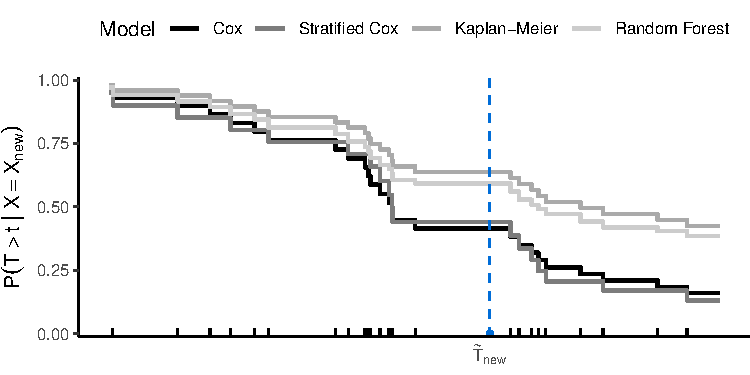
\includegraphics[width=0.9\textwidth]{./sl-hold-out-sample.pdf}
\end{center}
\end{onlyenv}
\end{frame}


\begin{frame}[label={sec:orgf238532}]{Existing approaches}
\small
\begin{block}{\normalsize Negative log-likelihood loss function \footnotesize (e.g., \cite{polley2011-sl-cens})}
Requires discrete time or modeling of a Lebesgue hazard function.

\hfill
\end{block}

\begin{block}{\normalsize Pseudo-observations \footnotesize (e.g., \cite{sachs2019ensemble})}
Requires pre-specification of an estimator of the censoring mechanism.

\hfill
\end{block}

\begin{block}{\normalsize IPCW \footnotesize (e.g., \cite{graf1999assessment,hothorn2006survival,gerds2006consistent,gonzalez2021stacked})}
Requires pre-specification of an estimator of the censoring mechanism.

\hfill
\end{block}

\begin{block}{\normalsize Iterative IPCW \footnotesize (\cite{westling2021inference,han2021inverse})}
Theoretical guarantees?
\end{block}
\end{frame}


\section{Proposal: The state learner}
\label{sec:orgc404b90}
\begin{frame}[label={sec:orge08b0a2}]{Proposal: Model the states of the \emph{observed} data}
\begin{onlyenv}<1>
\begin{block}{\centering \color{white} \((X, T) \sim Q\)}
\begin{center}
\includegraphics[width=.9\linewidth]{/tmp/babel-q4X6IR/figure-vDga9Y.pdf}
\end{center}
\end{block}
\end{onlyenv}

\begin{onlyenv}<2>
\begin{block}{\centering \((X, T) \sim Q\)}
\begin{center}
\includegraphics[width=.9\linewidth]{/tmp/babel-q4X6IR/figure-8pG1XI.pdf}
\end{center}
\end{block}
\end{onlyenv}

\begin{onlyenv}<3>
\begin{block}{\centering \color{darkgray}\((X, \tilde T, \Delta) \sim P\)\color{black}}
\begin{center}
\includegraphics[width=.9\linewidth]{/tmp/babel-q4X6IR/figure-NRCHP8.pdf}
\end{center}
\end{block}
\end{onlyenv}
\end{frame}


\begin{frame}[label={sec:org83a22d1}]{Conditional state-occupation probabilities for observed data}
\small

Define
% Record the observed data as \( O = (X, \{\eta(t) : t \geq 0\}) \), where
\begin{equation*}
  \eta(t) = \1{\{\tilde{T} \leq t, \Delta = 1\}} + 2 \, \1{\{\tilde{T} \leq t,
    \Delta = 0\}}
  \in \{0, 1, 2\},
\end{equation*}
and
\begin{equation*}
  F(t, j, x) = P(\eta(t) = j \mid X=x), \quad \text{for all } t \geq 0,\; j
  \in \{0, 1, 2\}, \; x \in \R^d.
\end{equation*}

\vfill

\begin{columns}
\begin{column}{0.45\columnwidth}
\centering \color{bblue}\(O = (X, \tilde T , \Delta)\)\color{black} 

\begin{center}
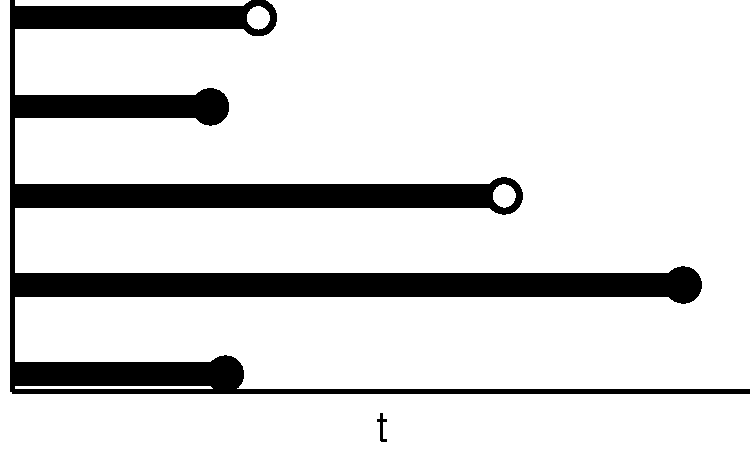
\includegraphics[width=0.9\textwidth]{./multi-state-data-1.pdf}
\end{center}
\end{column}

\begin{column}{0.45\columnwidth}
\centering \color{bblue}\(O = (X, \{\eta(t) : t \geq 0\})\)\color{black}

\begin{center}
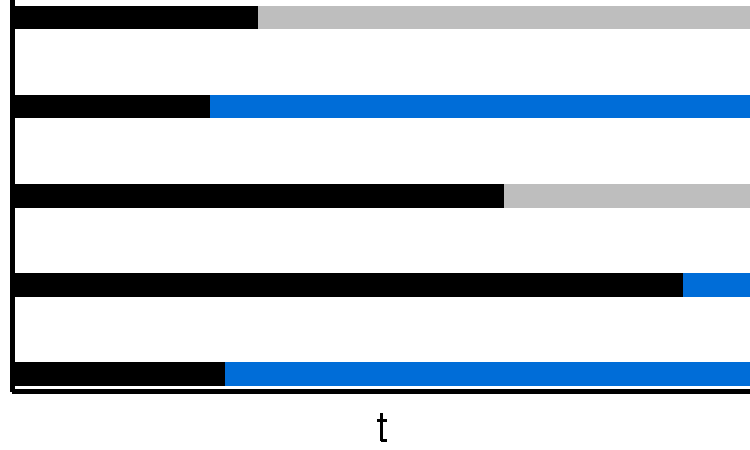
\includegraphics[width=0.9\textwidth]{./multi-state-data-3.pdf}
\end{center}
\end{column}
\end{columns}
\end{frame}

\begin{frame}[label={sec:org4a9f98d}]{The state learner}
\small

\begin{equation*}
  F(t, j, x) = P(\eta(t) = j \mid X=x), \quad \text{for all } t \geq 0,\; j
  \in \{0, 1, 2\}, \; x \in \R^d.
\end{equation*}

\vfill

The state learner is a super learner of \(F\).

\vfill

Performance can be evaluated using, e.g., the integrated Brier score
\( \bar{B}_{\tau}(F, O) = \int_0^{\tau} B_t(F, O) \diff t \), where
\begin{equation*}
  B_t(F, O) = \sum_{j=0}^{2} (F(t, j, X) - \eta(t))^2.
\end{equation*}

\vfill

Loss function does not depend on unknown nuisance parameters.

\vfill

No modeling of Lebesgue hazards or densities required.
\end{frame}

\begin{frame}[label={sec:org9a8d04e}]{Expressing \(F\) using \(\Lambda\) and \(\Gamma\)}
\small

\begin{equation*}
\begin{split}
F(t, 1, x)
& = P(\tilde{T} \leq t, \Delta=1 \mid X=x)
  = \int_0^t e^{-\Lambda(s \mid x) - \Gamma(s \mid x) }  \Lambda(\diff s \mid x),
\\
F(t, 2, x)
& = P(\tilde{T} \leq t, \Delta=0 \mid X=x)
  = \int_0^t e^{-\Lambda(s \mid x) - \Gamma(s \mid x) }  \Gamma(\diff s \mid x),
\\
F(t, 0, x)
&
  = P(\tilde{T} > t \mid X= x)
  = 1- F(t, 1, x) - F(t, 2, x).
\end{split}
\end{equation*}

\vspace{.5cm}

\begin{columns}
\begin{column}{0.45\columnwidth}
\centering \(\eta(t) : t \geq 0\)

\begin{center}
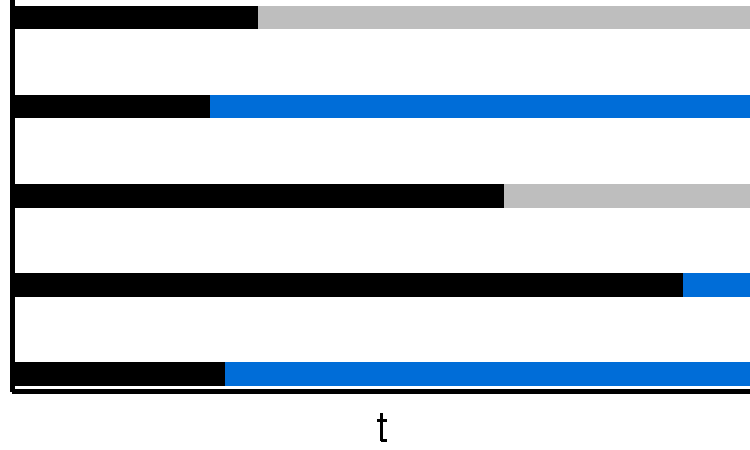
\includegraphics[width=0.9\textwidth]{./multi-state-data-3.pdf}
\end{center}
\end{column}

\begin{column}{0.5\columnwidth}
\begin{center}
\includegraphics[width=.9\linewidth]{/tmp/babel-q4X6IR/figure-Rf0nt3.pdf}
\end{center}
\end{column}
\end{columns}
\end{frame}

\begin{frame}[label={sec:org392cea0}]{Constructing a library for learning \(F\)}
\small

Given libraries \( \mathcal{A} \) and \( \mathcal{B} \) for learning $\Lambda$
and $\Gamma$, respectively,  define
\begin{equation*}
  \mathcal{F}(\mathcal{A}, \mathcal{B})
  = \{ \phi_{a, b} : a \in \mathcal{A}, b \in \mathcal{B}\},
\end{equation*}
where
\begin{align*}
  \phi_{a, b}(\mathcal{D}_n)(t,1,x) &= \int_0^t e^{-a(\mathcal{D}_n)(s \mid
    x) -
    b(\mathcal{D}_n)(s \mid x) }  a(\mathcal{D}_n)(\diff s \mid x),
  \\
  & \dots 
\end{align*}

\vfill

Evaluate performance of
\( \phi_{a, b} \in \mathcal{F}(\mathcal{A}, \mathcal{B}) \) as
\begin{equation*}
  \hat{R}_n(\phi_{a, b}; \bar{B}_{\tau}) =
  \frac{1}{K}\sum_{k=1}^{K}
  \frac{1}{| \mathcal{D}_n^{k} |}\sum_{O_i \in \mathcal{D}_n^{k}}
  \int_0^{\tau} \sum_{j=0}^{2} 
  \left\{
    \phi_{a, b}(\mathcal{D}_n^{-k})(t,j, X_i) - \eta_i(t)
  \right\}^2 \diff t.
\end{equation*}
\end{frame}

\begin{frame}[label={sec:orgfde3b31}]{Extension to competing risks setting}
\small

\begin{center}
\includegraphics[width=.9\linewidth]{/tmp/babel-q4X6IR/figure-1C6wEk.pdf}
\end{center}

\begin{equation*}
  \eta(t) = \1{\{\tilde{T} \leq t, \tilde{D} = 1\}} +
  2 \, \1{\{\tilde{T} \leq t, \tilde{D} = 2\}}
  +
  3 \, \1{\{\tilde{T} \leq t, \tilde{D} = 0\}}.
\end{equation*}
\begin{align*}
  F(t, 1, x)
  & = P(\tilde{T} \leq t, \tilde{D}=1 \mid X=x)
    = \int_0^t e^{-\Lambda_1(s \mid x) -\Lambda_2(s \mid x) - \Gamma(s \mid x) }  \Lambda_1(\diff s \mid x),
  \\
  & \dots
\end{align*}
\begin{equation*}
  \mathcal{F}(\mathcal{A}_1,\mathcal{A}_2, \mathcal{B})
  = \{ \phi_{a_1, a_2, b} : a_1 \in \mathcal{A}_1, a_2 \in \mathcal{A}_2, b \in \mathcal{B}\},
\end{equation*}
\end{frame}

\begin{frame}[label={sec:orgb6fa0a6},fragile]{Prototype\footnote{\url{https://github.com/amnudn/statelearner}}}
 \begin{onlyenv}<1>
\lstset{language=r,label= ,caption= ,captionpos=b,numbers=none}
\begin{lstlisting}
library(riskRegression)
data(Melanoma, package="riskRegression")
setDT(Melanoma)
head(Melanoma)
\end{lstlisting}

\begin{verbatim}
   time status                    event invasion ici      epicel       ulcer thick    sex age   logthick
1:   10      2       death.other.causes  level.1   2     present     present  6.76   Male  76  1.9110229
2:   30      2       death.other.causes  level.0   0 not present not present  0.65   Male  56 -0.4307829
3:   35      0                 censored  level.1   2 not present not present  1.34   Male  41  0.2926696
4:   99      2       death.other.causes  level.0   2 not present not present  2.90 Female  71  1.0647107
5:  185      1 death.malignant.melanoma  level.2   2     present     present 12.08   Male  52  2.4915512
6:  204      1 death.malignant.melanoma  level.2   2 not present     present  4.84   Male  28  1.5769147
\end{verbatim}
\end{onlyenv}

\begin{onlyenv}<2>
\lstset{language=r,label= ,caption= ,captionpos=b,numbers=none}
\begin{lstlisting}
library(glmnet)
library(randomForestSRC)
lib <- list(
  cox = list(model = "cox", x_form = ~sex+age+logthick),
  cox_penalty = list(model = "GLMnet", x_form = ~invasion+ici+epicel+ulcer+sex+age+logthick),
  km = list(model = "cox", x_form = ~1),
  cox_strat = list(model = "cox", x_form = ~strata(epicel)),
  rf = list(model = "rfsrc", x_form = ~invasion+ici+epicel+ulcer+sex+age+logthick, ntree = 50)
)
\end{lstlisting}
\end{onlyenv}

\begin{onlyenv}<3>
\lstset{language=r,label= ,caption= ,captionpos=b,numbers=none}
\begin{lstlisting}
set.seed(111)
sl = statelearner(learners = list(cause1 = lib,
				  cause2 = lib,
				  censor = lib),
		  data = Melanoma,
		  time = 5*365.25)
\end{lstlisting}

\lstset{language=r,label= ,caption= ,captionpos=b,numbers=none}
\begin{lstlisting}
sl$cv_fit
\end{lstlisting}

\begin{verbatim}
        cause1      cause2      censor     loss b
  1:        rf          km         cox 239.6142 1
  2:        rf          km cox_penalty 239.8218 1
  3:        rf          km          km 239.8678 1
  4:        rf cox_penalty         cox 239.9478 1
  5:        rf          km          rf 239.9732 1
 ---                                             
121: cox_strat         cox          km 258.8383 1
122:        km         cox cox_penalty 259.0642 1
123: cox_strat         cox   cox_strat 259.0704 1
124:        km         cox          km 259.1725 1
125:        km         cox   cox_strat 259.3449 1
\end{verbatim}
\end{onlyenv}
\end{frame}

\begin{frame}[label={sec:org71751bc}]{Some theoretical results}
\small \pause

\begin{block}{Strictly proper scoring rule}
We have that
\begin{equation*}
  F_P = \argmin_{F} P{[ \bar{B}_{\tau}(F, \blank)]},
\end{equation*}
for
\begin{equation*}
  F_P(t, j, x) = P(\eta(t) = j \mid X=x).
\end{equation*}

\hfill \pause
\end{block}

\begin{block}{Finite sample guarantee\footnote{\cite{van2003unicv,van2006oracle}}}
For all $\delta > 0$ and $n \in \N$,
\begin{align*}
  \E_{P}{\left[ \Vert \hat{\phi}_n(\mathcal{D}_n^{-k}) - F_P \Vert_{P}^2 \right]}
  & \leq (1 + 2\delta)
    \E_{P}{\left[ \Vert \tilde{\phi}_n(\mathcal{D}_n^{-k}) - F_P \Vert_{P}^2 \right]}
  \\
  & \quad
    + (1+ \delta) 16   K \tau
    \left(
    13 + \frac{12}{\delta}
    \right)
    \frac{\log(1 + |\mathcal{F}_n|)}{n}.
\end{align*}
\end{block}
\end{frame}

\begin{frame}[label={sec:org243659a}]{Proof of concept}
\small

Wrongly assuming (completely) independent censoring can lead to poor performance
of IPCW based super learner.

\begin{center}
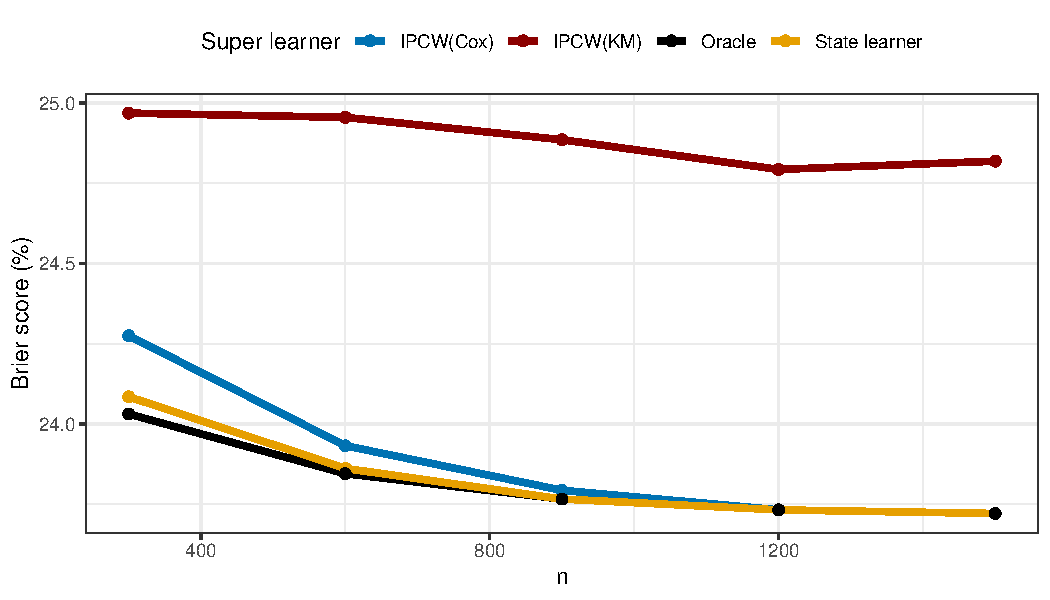
\includegraphics[width=.9\textwidth]{./ipcw-fail.pdf}
\end{center}
\end{frame}

\begin{frame}[label={sec:org70f1b5b}]{Illustration on real data with competing risks\footnote{Data from a prostate cancer studied by \cite{kattan2000pretreatment}.}}
\begin{center}
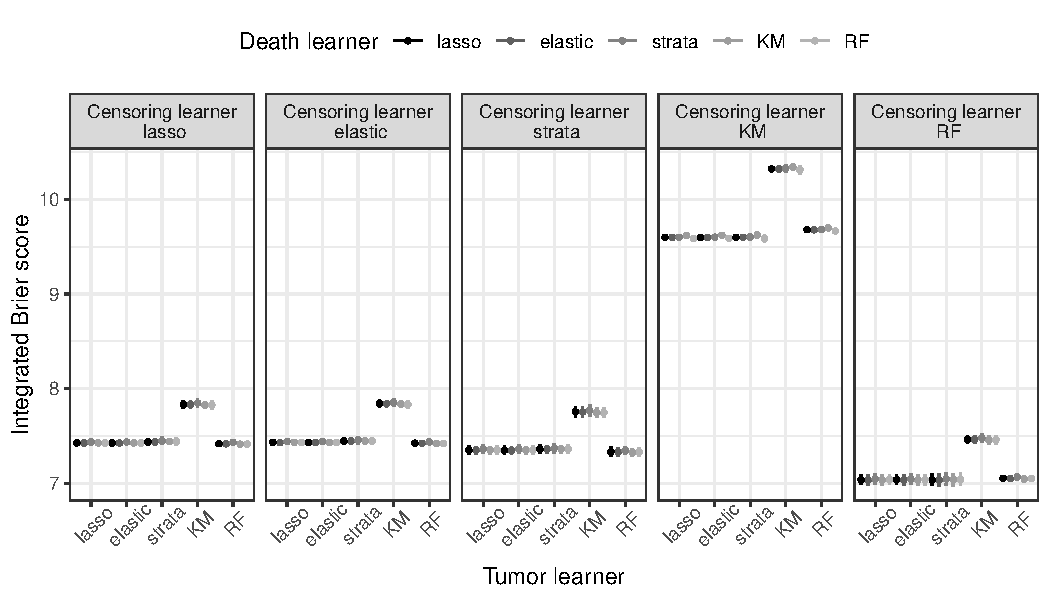
\includegraphics[width=1\textwidth]{./zelefski-real-data.pdf}
\end{center}
\end{frame}

\begin{frame}[label={sec:org7a41b07}]{Use with targeted learning}
\begin{block}{\centering \(F \longleftrightarrow (\Lambda, \Gamma)\)}
\begin{equation*}
  \Lambda(t \mid x) = \int_0^t \frac{F(\diff s, 1, x)}{F(s-, 0, x)} ,
  \quad \text{and} \quad
  \Gamma(t \mid x) = \int_0^t \frac{F(\diff s, 2, x)}{F(s-, 0, x)} .
\end{equation*}
\end{block}

\begin{block}{}
The efficient influence function for \(\tilde{\Psi}_t\) can be indexed by
\((\Lambda, \Gamma)\) or \(F\).
\end{block}

\begin{block}{}
The output from the state learner can be applied to construct a targeted
estimator.
\end{block}
\end{frame}

\begin{frame}[label={sec:org8a1315d}]{Second order remainder term}
Important property that
\begin{equation*}
  \text{Rem}(\hat{P}_n, P) = \Psi(P) - \Psi(\hat{P}_n) - P{[
    \psi(\blank, \hat{P}_n)]}
\end{equation*}
is of second order.

\vfill

For survival problems, \( \text{Rem}(\hat{P}_n, P) \) is typically dominated
by terms of the form
\begin{equation*}  
  \E_P{\left[ \int_0^t \hat{w}(s, X) \hat{M}_1(s \mid X)  \hat{M}_2(\diff s \mid X)] \right]},
\end{equation*}
where \( \hat{M}_j \) is either \( [\Lambda - \hat{\Lambda}_n] \) or
\( [\Gamma - \hat{\Gamma}_n ]\).
\end{frame}



\begin{frame}[label={sec:orgccfb162}]{Second order remainder with the state learner}
Second order property remains, in the sense that the remainder is dominated by
terms of the form,
\begin{equation*}  
  \E_P{\left[ \int_0^t
      \hat{w}_*(s, X) [F - \hat{F}](s-, j, X)  [F- \hat{F}](\diff s, j', X)] \right]},
\end{equation*}

\vfill

Second order in terms of convergence rate.
\end{frame}



\section{Discussion}
\label{sec:org10c1928}
\begin{frame}[label={sec:org8f9f393}]{Ongoing work}
Extension to continuous super learner. How to best construct a convex
combination?
\begin{equation*}
  \sum_{(a, b)} \alpha_{a,b} \phi_{a, b},
  \quad \text{or} \quad 
  \phi_{\sum_a w_a a, \sum_b w_b b}, 
\end{equation*}
where
\begin{align*}
  \phi_{a, b}(\mathcal{D}_n)(t,1,x) &= \int_0^t e^{-a(\mathcal{D}_n)(s \mid
    x) -
    b(\mathcal{D}_n)(s \mid x) }  a(\mathcal{D}_n)(\diff s \mid x),
  \\
  & \dots 
\end{align*}


\vfill

Simulation study to assess effect on low-dimensional target parameters.

\vfill

Better implementation. Make more learners available.
\end{frame}

\begin{frame}[label={sec:orgdb37af7}]{Discussion and open questions}
Limitation that \(F\) is a feature of the observed data distribution.
Important whether we estimate \(F\) or \((\Lambda, \Gamma)\) when the
parameter of interest is \(\Psi \colon \mathcal{P} \rightarrow \R\)?

\vfill

Second order remainder in terms of rates. Some double robustness property might
be lost. Relying too much on good estimation of all of \(F\)?

\vfill

Can we build or good risk prediction from the state learner?

\vfill

Will a targeted estimator based on the state learner be robust against or
sensitive to near positivity violations?
\end{frame}

\begin{frame}[label={sec:orgdbdd600}]{Summary}
\begin{itemize}
\item Aim to avoid the need to pre-specify a censoring model.
\item Select a tuple (or triple) of learners \((\Lambda, \Gamma)\) jointly optimal
for predicting the states occupied by the observed data
\item No need to estimate additional nuisance parameters in the hold-out sample.
\item No need to model Lebesgue densities or hazards.
\item Drawback that the state learner is tuned for the a feature of the observed
data distribution.
\end{itemize}
\end{frame}

\section*{References}
\label{sec:orgb1961be}
\begin{frame}[label={sec:orged3ce61}]{References}
\tiny \bibliography{./latex-settings/default-bib.bib}
\end{frame}
\end{document}